\documentclass[12pt]{article}
\usepackage{fullpage,enumitem,amsmath,amssymb,graphicx,grffile,float,listings}



\begin{document}
    %Title Section
    \begin{flushleft}
    \LARGE CS229 Fall 2017\\
    \LARGE Problem Set \#1: Supervised Learning\\
    \textbf{\normalsize Author: LFhase \quad rimemosa@163.com}
    \end{flushleft} 
    \noindent
    \rule{\linewidth}{0.4pt}
    %Title Section

    %Problem and Solution

    \section*{Logistic regression  }

    \begin{enumerate}[label=(\alph*)]

    \item 
    {
        Given that \\
        $$J(\theta)= \frac{1}{m} \sum_{i=1}^{m}log(1+e^{-y^{(i)}\theta^{T}x^{(i)}})$$\\
        we can get
        $$\frac{\partial J(\theta)}{\partial \theta_{i}}
            =  \frac{1}{m} \sum_{k=1}^{m} \frac{-y^{(k)}x^{(k)}_i}{1+e^{y^{(k)}\theta^{T}x^{(k)}}}
        $$\\
        then
        $$\frac{\partial J(\theta)}{\partial \theta_{i} \partial \theta_{j}}
            =  \frac{1}{m} \sum_{k=1}^{m} 
            \frac{x^{(k)}_ix^{(k)}_je^{y^{(k)}\theta^{T}x^{(k)}}}
            {(1+e^{y^{(k)}\theta^{T}x^{(k)}})^2}
        $$\\
        which is $ H_{ij} $\\
        so
        \begin{equation*} 
        \begin{split}
            Z^THZ &= \sum_{i=1}^n \sum_{j=1}^n z_iH_{ij}z_j \\
            &= \frac{1}{m} \sum_{k=1}^{m} 
            \frac{\sum_{i=1}^n \sum_{j=1}^n z_ix^{(k)}_ix^{(k)}_jz_je^{y^{(k)}\theta^{T}x^{(k)}}}{(1+e^{y^{(k)}\theta^{T}x^{(k)}})^2}
            \\
        \end{split}
        \end{equation*} 
        known that 
        $$ \sum_{i=1}^n \sum_{j=1}^n z_ix^{(k)}_ix^{(k)}_jz_j = (X^TZ)^2 \geq 0 $$\\
        $$ \frac{e^{y^{(k)}\theta^{T}x^{(k)}}}{(1+e^{y^{(k)}\theta^{T}x^{(k)}})^2} > 0 $$\\
        we can easily get $$ Z^THZ \geq 0 $$
    }
    \newpage
    \item 
    {
        Firstly, we plot the original data \\

        \begin{figure}[H]
            \centering
            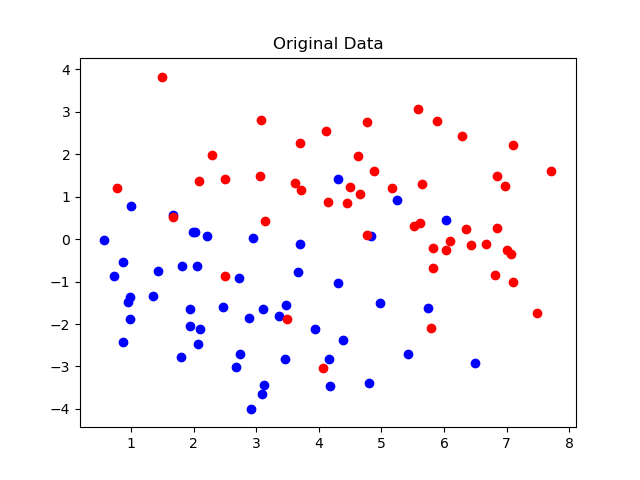
\includegraphics[width=0.80\textwidth]{figure/original_data.png}
        \end{figure}

        To implement Newton’s Method, we calculate the value of 
        $$\frac{1}{m} \sum_{k=1}^{m} \frac{-y^{(k)}x^{(k)}_i}{1+e^{y^{(k)}\theta^{T}x^{(k)}}}
        $$
        and $\textbf{Hessian}$\\
        then using the \textbf{update rule}
        $$ \theta := \theta - H^{-1}\bigtriangledown_\theta l(\theta) $$
    }
    
    \newpage
    \item 
    {
        Through 6 iterations, we finally get the result
        \begin{figure}[H]
            \centering
            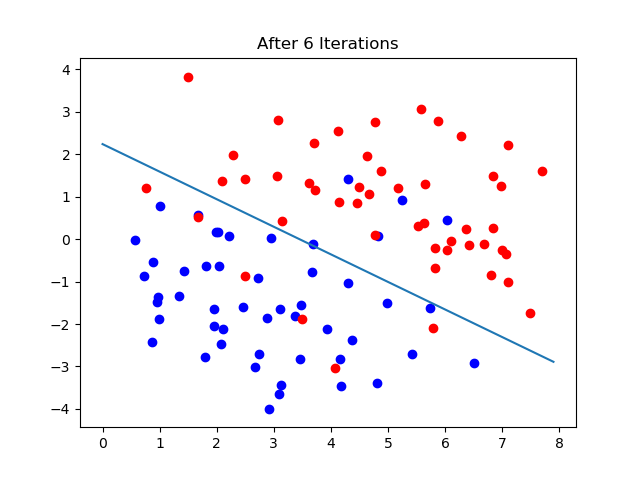
\includegraphics[width=0.80\textwidth]{figure/Iteration6.png}
        \end{figure}
        and the $ \theta $ is  [-2.6205116,   0.76037154,  1.17194674].
    }

    \end{enumerate}


\end{document}